\chapter{Stadiul actual și analiza tehnologiilor}

\section{De la HTTP la MQTT: comunicația în IoT}
La prima vedere, un microcontroler care raportează date către un server este o aplicație web ca oricare alta. În realitate, dacă încercăm să folosim HTTP/REST pentru un nod IoT, costurile devin rapid prohibitive.

Modelul cerere-răspuns presupune că senzorul deschide o conexiune TCP nouă pentru fiecare mesaj, trimite un header HTTP care, cu cookie-uri și meta-informații, poate ajunge la câteva sute de bytes, apoi așteaptă răspunsul și închide conexiunea. Atunci când serverul vrea să trimită o comandă către dispozitiv, problema se mută: HTTP nu suportă push nativ, deci fie clientul interoghează ciclic (\textit{polling}), fie se trece la WebSocket-uri, ceea ce ne aduce, de fapt, foarte aproape de paradigma de \textit{publish/subscribe}.

MQTT alege o cale diferită. Există un broker central, iar fiecare client (senzor sau aplicație) menține o singură conexiune TCP persistentă cu el. Mesajele se publică pe „topice” — șiruri ierarhice de forma \texttt{homeforge/devices/AABBCCDDEEFF/state} — iar brokerul rutează automat fiecare publicare către toți abonații topicului respectiv. Antetul minim al unui pachet MQTT este de doar 2 bytes \cite{mqtt_standard_iot}, iar protocolul oferă nativ trei niveluri de QoS și un mecanism de \textit{Last Will and Testament}, prin care brokerul detectează automat deconectarea unui nod.

Naik a evaluat comparativ patru protocoale de mesagerie pentru IoT (MQTT, CoAP, AMQP și HTTP) și a arătat că MQTT și CoAP sunt mai potrivite pentru rețele de senzori cu lățime de bandă redusă și noduri cu resurse limitate, în timp ce HTTP rămâne natural pentru integrări cu sisteme web tradiționale \cite{mqtt_vs_http_iot_perf}. Mishra și Kertész, în survey-ul lor extensiv asupra MQTT în M2M și IoT, listează implementări de broker (Mosquitto, HiveMQ, EMQ X, VerneMQ) și concluzionează că Mosquitto este una dintre cele mai populare alegeri datorită amprentei mici și a faptului că rulează inclusiv pe Raspberry Pi \cite{mqtt_standard_iot}.

\begin{figure}[htbp]
    \centering
    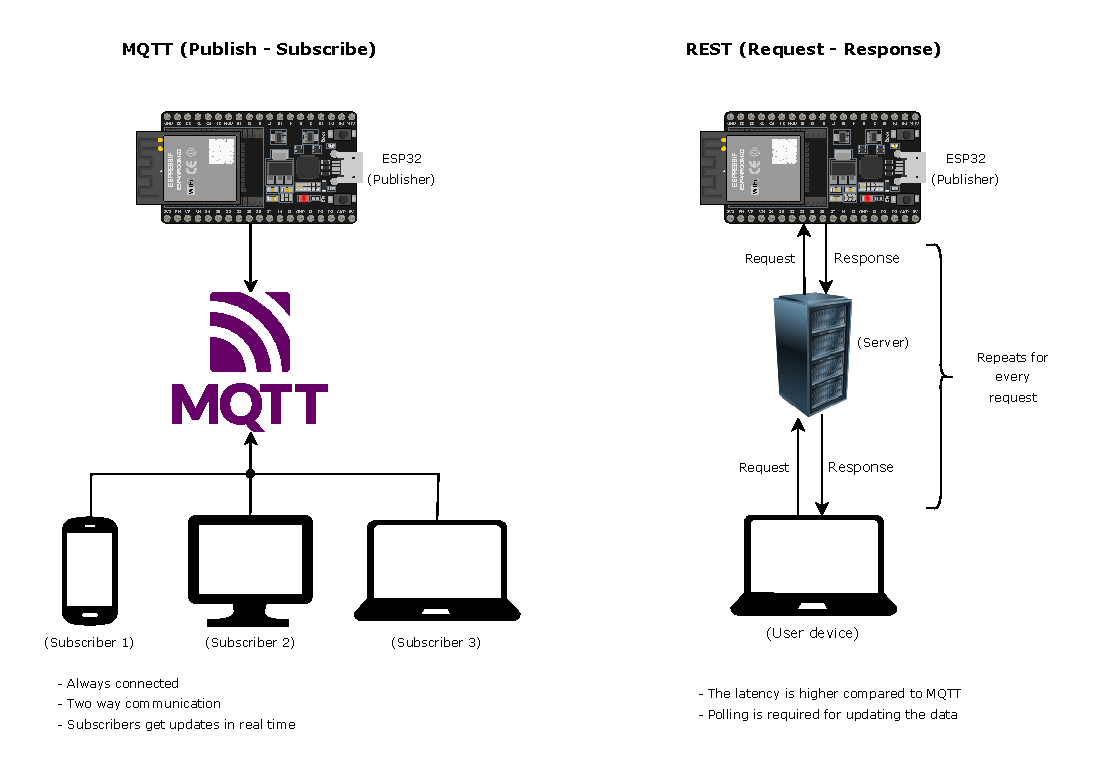
\includegraphics[width=0.9\textwidth]{figuri/MQTT_vs_REST.pdf}
    \caption{Comparație arhitecturală între modelul HTTP cerere-răspuns și modelul \textit{publish/subscribe} bazat pe MQTT}
    \label{fig:mqtt_vs_http}
\end{figure}

În HomeForge folosesc o abordare hibridă, pentru că fiecare protocol are zona în care este eficient:
\begin{itemize}
    \item MQTT pentru comunicația cu dispozitivele fizice — telemetrie și comenzi, în timp real;
    \item HTTP/REST pentru interacțiunea browser--backend — fetch-ul listei de dispozitive, login, profil, layout-ul dashboard-ului.
\end{itemize}
Frontend-ul nu vorbește direct cu brokerul MQTT; el comunică doar cu API-ul REST al Django, iar backend-ul este cel care traduce între cele două lumi.

\begin{table}[htbp]
    \centering
    \caption{MQTT vs. HTTP/REST în context IoT}
    \vspace{0.4\baselineskip}
    \label{tab:mqtt_vs_rest}
    {\setstretch{1.0}
    \footnotesize
    \renewcommand{\arraystretch}{1.15}
    \begin{tabular}{|>{\raggedright\arraybackslash}p{3.2cm}|>{\raggedright\arraybackslash}p{5.8cm}|>{\raggedright\arraybackslash}p{5.8cm}|}
        \hline
        \textbf{Caracteristică} & \textbf{MQTT} & \textbf{HTTP / REST} \\ \hline
        Model & Asincron, \textit{publish-subscribe} (broker) & Sincron, cerere-răspuns \\ \hline
        Overhead antet & de la 2 bytes & sute de bytes (headere, cookies) \\ \hline
        Conexiune TCP & Persistentă (\textit{stateful}) & Per cerere (\textit{stateless}) \\ \hline
        QoS nativ & Da, 3 niveluri & Nu (depinde de aplicație) \\ \hline
        Push server $\rightarrow$ client & Suportat nativ & Necesită \textit{polling} sau WebSocket-uri \\ \hline
        Caz tipic & Telemetrie, microcontrolere & API web, operații CRUD \\ \hline
    \end{tabular}
    }
\end{table}

\section{Platforme open-source: unde se poziționează HomeForge}
Soluțiile open-source dedicate Smart Home-ului sunt deja mature. Cele mai cunoscute, Home Assistant și OpenHAB, au câștigat o tracțiune semnificativă în comunitate prin integrările cu sute de producători, prin suportul pentru protocoale specializate (Zigbee, Z-Wave, KNX, Matter), prin reguli avansate de automatizare construite vizual și prin documentația vastă creată de utilizatori.

Pentru un utilizator final care vrea o casă inteligentă completă, oricare dintre ele este o alegere mai bună decât HomeForge. Diferența este nișa în care lucrăm. HomeForge nu vrea să suporte 100 de producători, nici 10. Vrea să suporte un singur lucru bine: dispozitive făcute manual, pe ESP32, care vorbesc MQTT printr-un format JSON simplu. În schimb, oferă:
\begin{itemize}
    \item un cod sursă scurt (sub 2500 de linii pentru API-ul backend, vezi \texttt{views.py});
    \item zero magie ascunsă — fiecare endpoint este vizibil în \texttt{urls.py};
    \item un \textit{device builder} grafic, care permite construirea unui tip de dispozitiv vizual și exportă firmware-ul ESP32 corespunzător;
    \item o curbă de învățare scăzută pentru studenți, care pot extinde sistemul fără să citească arhitectura unei platforme cu 10 ani de dezvoltare în spate.
\end{itemize}

Cu alte cuvinte, HomeForge nu intră în competiție cu Home Assistant pe terenul lui. Acoperă o zonă diferită: a celui care vrea să prototipeze rapid, să înțeleagă fluxul de date end-to-end și, eventual, să pornească de aici către un sistem mai serios.

\section{Justificarea stivei tehnologice}
Alegerile tehnologice nu sunt accidentale: fiecare componentă rezolvă o problemă concretă pe care am întâlnit-o în implementare. Mai jos justific principalele opțiuni; ele se vor regăsi în capitolele de implementare.

\subsection{Backend: Python, Django și DRF}
Python a fost ales pentru că oferă cele mai mature biblioteci pentru manipularea datelor heterogene (\texttt{paho-mqtt}, \texttt{Pillow}, \texttt{ArduinoJson} la nivel de embed). Django adaugă peste asta un ORM matur, un sistem de migrații versionabil și protecții implicite împotriva atacurilor uzuale (CSRF, XSS, SQL injection). Django REST Framework completează stack-ul cu \textit{serializers}, \textit{viewsets} și \textit{permission classes}, care reduc semnificativ codul boilerplate atunci când construiești un API.

Concret, în HomeForge, un endpoint precum \texttt{POST /api/devices/} este descris în doar câteva zeci de linii, validările sunt declarate în serializer, iar permisiunile sunt asignate per view (vezi \texttt{views.py:376-461}).

\subsection{Bază de date: PostgreSQL cu JSONB}
La nivel de bază de date, am avut nevoie de două lucruri în același loc: relații stricte (un dispozitiv aparține unui utilizator și opțional unei camere) și structuri flexibile (starea curentă a unui dispozitiv este JSON arbitrar). PostgreSQL este unul dintre puținele RDBMS-uri care oferă bine ambele lumi, prin tipul \texttt{JSONB} și suport pentru indexare GIN.

Documentația oficială PostgreSQL precizează că, spre deosebire de tipul \texttt{json} (care păstrează textul JSON brut), \texttt{JSONB} pre-parsează documentul într-un format binar decompus, ceea ce face citirea ulterioară mai rapidă și permite indexare cu \texttt{GIN} pentru căutări în interiorul JSON-ului \cite{postgresql_jsonb_docs}. Pentru o platformă didactică, această combinație este ideală: studenții văd o schemă SQL clară pentru \texttt{User}, \texttt{Room}, \texttt{Device}, dar nu sunt obligați să facă o migrație de fiecare dată când adaugă un senzor cu un format nou.

În cod, decizia se traduce într-un singur câmp:
\begin{minted}{python}
class Device(models.Model):
    # ... relațiile clasice ...
    current_state = models.JSONField(
        default=dict, blank=True,
        help_text="Current state of device controls"
    )
\end{minted}

\subsection{Magistrală de mesaje: MQTT (Mosquitto)}
Pentru implementarea concretă a brokerului, am folosit Mosquitto — open-source, standardizat OASIS, suficient de ușor încât poate rula în același container Docker cu backend-ul. Pe portul implicit 1883, brokerul ascultă atât de la clienții ESP32 cât și de la procesul \texttt{mqtt\_listener} al backend-ului.

În implementarea curentă, mecanismul \textit{Last Will and Testament} oferit de MQTT nu este utilizat; statusul \texttt{offline} este detectat printr-un timer aplicativ, în cadrul comenzii \texttt{mqtt\_listener} — un dispozitiv care nu a publicat în ultimele 30 de secunde este marcat ca \texttt{offline}. Această abordare simplifică firmware-ul ESP32 și centralizează logica de gestionare a stării în partea Python a aplicației.

\subsection{Frontend: React, Next.js și TanStack Query}
Pe partea de UI, dashboard-ul este un \textit{Single Page Application} care își actualizează cardurile în timp real, pe baza datelor preluate de la backend. React rezolvă re-randarea eficientă prin Virtual DOM, iar Next.js oferă deasupra un \texttt{app router} modern, suport \textit{Server-Side Rendering} (pe care nu îl folosesc agresiv în acest proiect) și un sistem de bundling deja optimizat — la combinarea celor două, ecuația practică e că obțin un timp scurt până la prima interacțiune fără să configurez manual Webpack sau alte unelte de build.

În HomeForge folosesc TanStack Query (fost React Query) pentru toată stocarea de date la nivel de client. Decizia este motivată de două lucruri: (1) cache automat și deduplicare a cererilor, (2) suport excelent pentru \textit{optimistic updates}, care este coloana vertebrală a UI-ului responsiv din dashboard. Detaliile sunt în Capitolul 4.

\subsection{Containerizare: Docker și Docker Compose}
Problema „pe calculatorul meu funcționează” este reală în orice proiect cu mai multe servicii. Bellavista și Zanni au demonstrat că este fezabil să rulezi containere Docker chiar și pe noduri Edge cu resurse limitate, cum este Raspberry Pi, ceea ce arată că aceeași imagine se poate distribui fără modificări de la un server la un nod de margine \cite{docker_iot_edge}. În HomeForge:
\begin{itemize}
    \item \texttt{backend} (Django + Mosquitto + Avahi) și \texttt{db} (PostgreSQL) rulează ca două servicii separate;
    \item \texttt{frontend} este al treilea container, cu o imagine Next.js standard;
    \item dezvoltatorul rulează totul cu \texttt{docker compose up}, fără să instaleze nimic local.
\end{itemize}
Pentru dezvoltare rapidă există și varianta \texttt{./dev.sh}, care pornește backend-ul și frontend-ul direct pe mașina gazdă, ocolind containerele.

% FIGURĂ DE ADĂUGAT: o diagramă verticală a stivei tehnologice:
% sus „Frontend (Next.js + React + TanStack Query)”,
% la mijloc „Backend (Django + DRF) + Broker MQTT (Mosquitto) + PostgreSQL”,
% jos „Hardware (ESP32 + senzori DHT11/BMP180 + relee)”.
% Poate fi desenată cu draw.io / Inkscape și exportată ca PDF.
\begin{figure}[htbp]
    \centering
    % 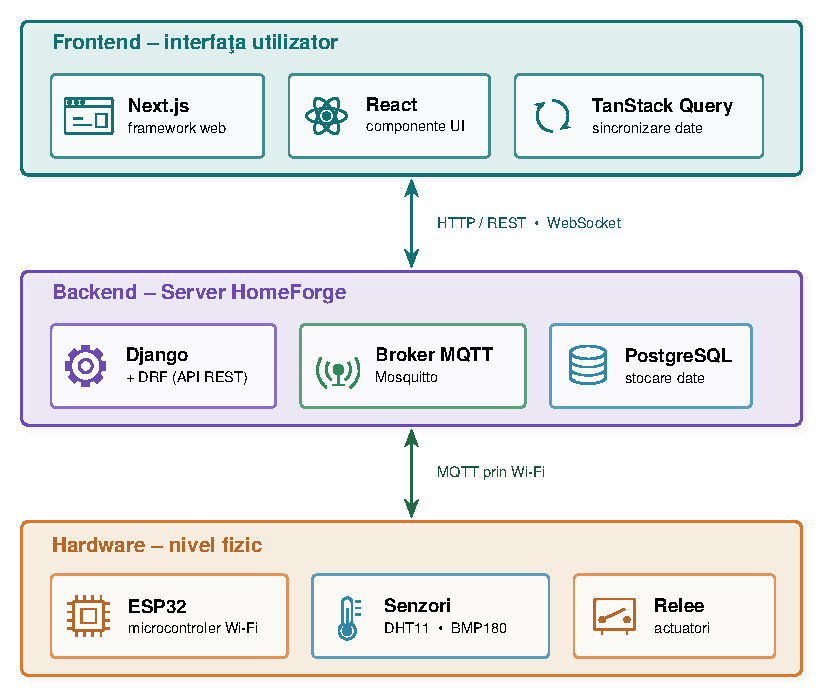
\includegraphics[width=0.7\textwidth]{figuri/stiva_tehnologica.pdf}
    \caption{Stiva tehnologică decuplată a platformei HomeForge (figură de adăugat)}
    \label{fig:tech_stack}
\end{figure}
